% Homework 11.tex 

\documentclass{article}
\usepackage{graphicx} % for figures
\usepackage{float}
\usepackage[export]{adjustbox}
\usepackage{fancyhdr}
\begin{document}

\title{Homework 11 - Physics 240\\
		System of Spring and Matrix Inversion}
\author{Tin Tran}

\maketitle

\section{Introduction}
The purpose of this excercise is to solve a system of spring using the matrix inversion method. The static solution of the system with 4 springs are given.\\
\indent What I did was basically hard code the matrix using the values given in the homework, I could have setup different arrays of k and L and then using the index to setup the matrix that way, but since we only have 6 matrix for the 6 k and L given, I decided to hard code 6 matrices. I then compute the values for Frw using the matrix and numerical method, and they all agree.**
\section{Discussion}
My physical argument for the 5 cases are as followed:\\
a) I get 0 for F, which makes sense, because the system is not moving.\\
b) I get -2.88 for F, this could mean that the system is moving to the right.\\
c) I get 0.5 for F, this means that the system is now moving the opposite direction.\\
d) I get 0.6 for F, this means that the system is still moving to the opposite direction.\\
e) I get -1 for F, this means the system now has changed the direction and moving to the right.\\

The plot I got looks like this:

\begin{figure}[H]
\centering{
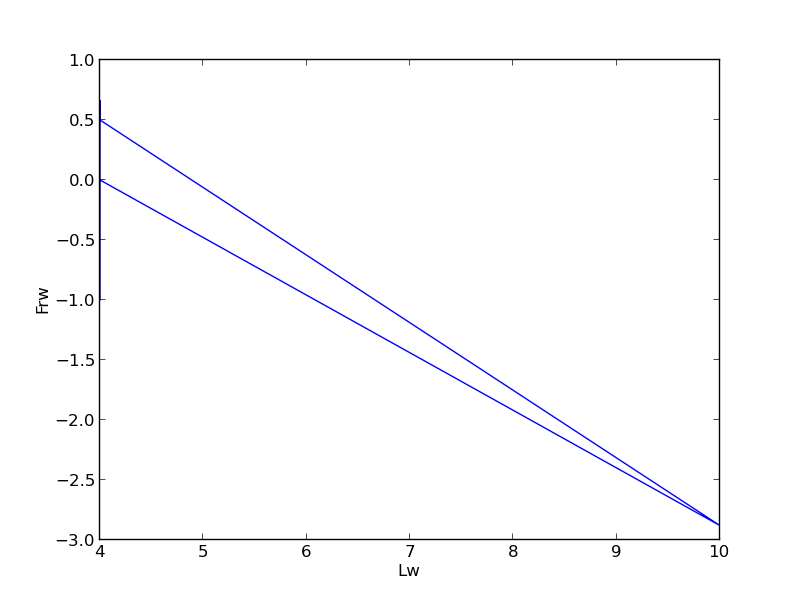
\includegraphics[max size={\textwidth}{\textheight}]{hw11.png}
\caption{Plot of F and Lw}
}
\end{figure}

I don't know what's wrong here since I can't make sense of this figure, what I did was to plot each value of F with the given values of Lw.\\\\
**note on the last matrix e, it was not invertable, I had to change k$_2$ from 1 to 0 for the first line, and so the calculated value was 0 whereas the numerical value is 0.6
\end{document}